% Compile: pdflatex -shell-escape diagram-methods.tex && dvisvgm --pdf --no-fonts diagram-methods.pdf
\documentclass[border=12pt]{standalone}
\usepackage{tikz}
\usetikzlibrary{arrows.meta, positioning, backgrounds}
\usepackage[sfdefault]{carlito}   % standard TikZ-ish sans font from TeX Live
\definecolor{card}{HTML}{FFFFFF}
\definecolor{ink}{HTML}{0F1730}
\definecolor{cyanA}{HTML}{0E7490}
\definecolor{violetA}{HTML}{6D28D9}
\definecolor{emeraldA}{HTML}{047857}
\definecolor{row}{HTML}{F1F5FB}
\begin{document}
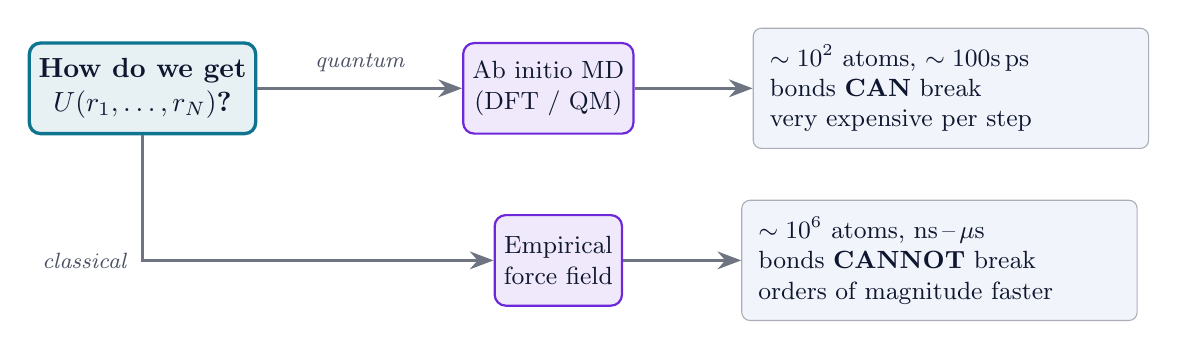
\begin{tikzpicture}[
  font=\small,
  q/.style={draw=cyanA, very thick, rounded corners=4pt, fill=cyanA!10, text=ink,
           align=center, minimum height=1.15cm, font=\bfseries},
  branch/.style={draw=violetA, thick, rounded corners=4pt, fill=violetA!10, text=ink,
           align=center, minimum height=1.15cm},
  ann/.style={draw=ink!35, rounded corners=3pt, fill=row, text=ink,
           align=left, inner sep=6pt},
  arr/.style={-{Stealth[length=3mm]}, very thick, color=ink!60},
  lab/.style={font=\footnotesize\itshape, text=ink!75}
]
  \node[q] (Q) {How do we get\\ $U(r_1,\dots,r_N)$?};

  \node[branch] (DFT) [right=2.6cm of Q] {Ab initio MD\\(DFT / QM)};
  \node[branch] (FF)  [below right=1.0cm and 2.6cm of Q, xshift=0.4cm] {Empirical\\ force field};

  \node[ann] (D) [right=1.5cm of DFT, text width=4.6cm] {
    $\sim 10^2$ atoms, $\sim 100$s\,ps\\
    bonds \textbf{CAN} break\\
    very expensive per step};
  \node[ann] (E) [right=1.5cm of FF, text width=4.6cm] {
    $\sim 10^6$ atoms, ns\,--\,$\mu$s\\
    bonds \textbf{CANNOT} break\\
    orders of magnitude faster};

  \draw[arr] (Q) -- (DFT) node[lab, midway, above=2pt] {quantum};
  \draw[arr] (Q) |- (FF) node[lab, midway, left=2pt] {classical};
  \draw[arr] (DFT) -- (D);
  \draw[arr] (FF) -- (E);
\end{tikzpicture}
\end{document}